\section{Ước lượng mức hiểu của học sinh}\label{sec:eval-learner}

Sau mỗi câu học sinh làm, hệ thống cập nhật điểm hiểu bài $M$ từ $0$ đến $100$ (gộp bốn khía cạnh chính: khái niệm $C$, lập luận $R$, vận dụng $A$, làm không cần gợi ý $I$), mức hiểu từ $0$ đến $5$, trạng thái qua bài và độ tin cậy (mục~\ref{sec:learner-design}). Điểm không do mô hình ngôn ngữ cho mà do công thức tính lại từ nhật ký, nên cùng nhật ký luôn cho cùng điểm. Đối chiếu hai mươi lăm mục của khung đánh giá Toán với mã nguồn cho $16$ mục làm đầy đủ, $5$ mục làm một phần và $4$ mục chưa làm, tức độ sát khung $74\%$ khi mục một phần tính một nửa và $64\%$ khi chỉ tính mục đầy đủ; các mục chưa làm xoay quanh thời gian, tức bài kiểm tra sau nhiều ngày để đo trí nhớ. Mục này bổ sung bốn loại bằng chứng: tính lại điểm từ nhật ký thật, kiểm tra công thức, thử với các kiểu học sinh biết trước và đo độ nhạy với các con số tự đặt.

\subsection{Tính lại điểm từ nhật ký của tài khoản Vuong}
Mỗi buổi được đưa vào công thức của chương mà nó đã dùng, đúng phiên bản chương lúc đó, rồi các buổi cùng chương được nối tiếp theo thời gian, đúng như trang giáo viên làm. Chương Số thập phân có năm buổi ngày 12 và 13/10, chương Diện tích có bốn buổi và Unit~11 có hai buổi ngày 15/11. Bảng~\ref{tab:db-mastery} cho trạng thái cuối. Cả ba chương đều qua mọi bài ($11/11$, $8/8$ và $6/6$) với điểm hiểu bài trung bình $87{,}0$, $86{,}5$ và $83{,}5$, mức hiểu trung bình $3{,}36$, $3{,}50$ và $3{,}67$; không bài nào đạt mức $5$ vì đợt thử nghiệm chưa đo trí nhớ. Ba khía cạnh khái niệm, vận dụng và làm không cần gợi ý đều từ $86{,}7$ trở lên, còn lập luận chỉ khoảng $74$ đến $75{,}5$, khớp với việc phần lớn câu ``vì sao'' ở Toán đạt $0{,}6$ chứ ít khi đạt $1{,}0$. Độ tin cậy trung bình chỉ khoảng $39$ đến $42$ trên một trăm: điểm đã vượt ngưỡng qua bài nhưng lượng bằng chứng chưa đủ để hệ thống coi kết luận là chắc, đúng nguyên tắc không phóng đại điều chưa đủ dữ liệu.

% Sinh bởi tools/db_learner.py từ bản sao lưu database; không sửa tay.
\begin{table}[H]
\centering
\caption{Trạng thái mức hiểu của tài khoản Vuong sau khi gấp mọi buổi của từng chương}\label{tab:db-mastery}
\begin{tabular}{lrrr}
\toprule
Chỉ số & Số thập phân & Diện tích & Tiếng Anh \\
\midrule
Số buổi đã gấp & $5$ & $4$ & $2$ \\
Số bài của chương & $11$ & $8$ & $6$ \\
Số bài đã qua & $11$ & $8$ & $6$ \\
Điểm hiểu bài $M$ trung bình & $87{,}0$ & $86{,}5$ & $83{,}5$ \\
Mức hiểu trung bình (thang $0$--$5$) & $3{,}36$ & $3{,}50$ & $3{,}67$ \\
Độ tin cậy trung bình & $41{,}6$ & $39{,}9$ & $38{,}7$ \\
Chiều khái niệm $C$ & $94{,}8$ & $95{,}5$ & $87{,}8$ \\
Chiều lập luận $R$ & $75{,}5$ & $74{,}1$ & $74{,}0$ \\
Chiều vận dụng $A$ & $97{,}6$ & $93{,}6$ & $86{,}7$ \\
Chiều độc lập $I$ & $89{,}9$ & $90{,}3$ & $88{,}0$ \\
\bottomrule
\end{tabular}
\end{table}


Hình~\ref{fig:db-mastery} cho điểm trung bình theo số buổi đã tính. Chương Số thập phân có cả mười một bài đã qua sau buổi đầu (điểm trung bình $90{,}9$) và ba buổi sau đưa điểm xuống $87{,}0$ vì các câu sai mới ghi thêm bằng chứng xấu, tức một bài đã qua vẫn có thể mất điểm. Buổi đầu của chương Diện tích chỉ có $12$ câu nên mới hai bài qua (điểm $76{,}5$) và buổi thứ hai đưa cả tám bài qua. Điểm cuối của từng bài nằm trong khoảng $80{,}7$ đến $92{,}9$ ở Số thập phân, $80{,}0$ đến $90{,}6$ ở Diện tích và $75{,}0$ đến $87{,}0$ ở Unit~11. Hệ thống theo dõi năm lỗi hiểu sai ở Số thập phân (một hoạt động, hai đang giải quyết, hai đã giải quyết), hai lỗi đã giải quyết ở Diện tích và sáu lỗi ở Unit~11 (năm đã giải quyết).

\begin{figure}[H]
\centering
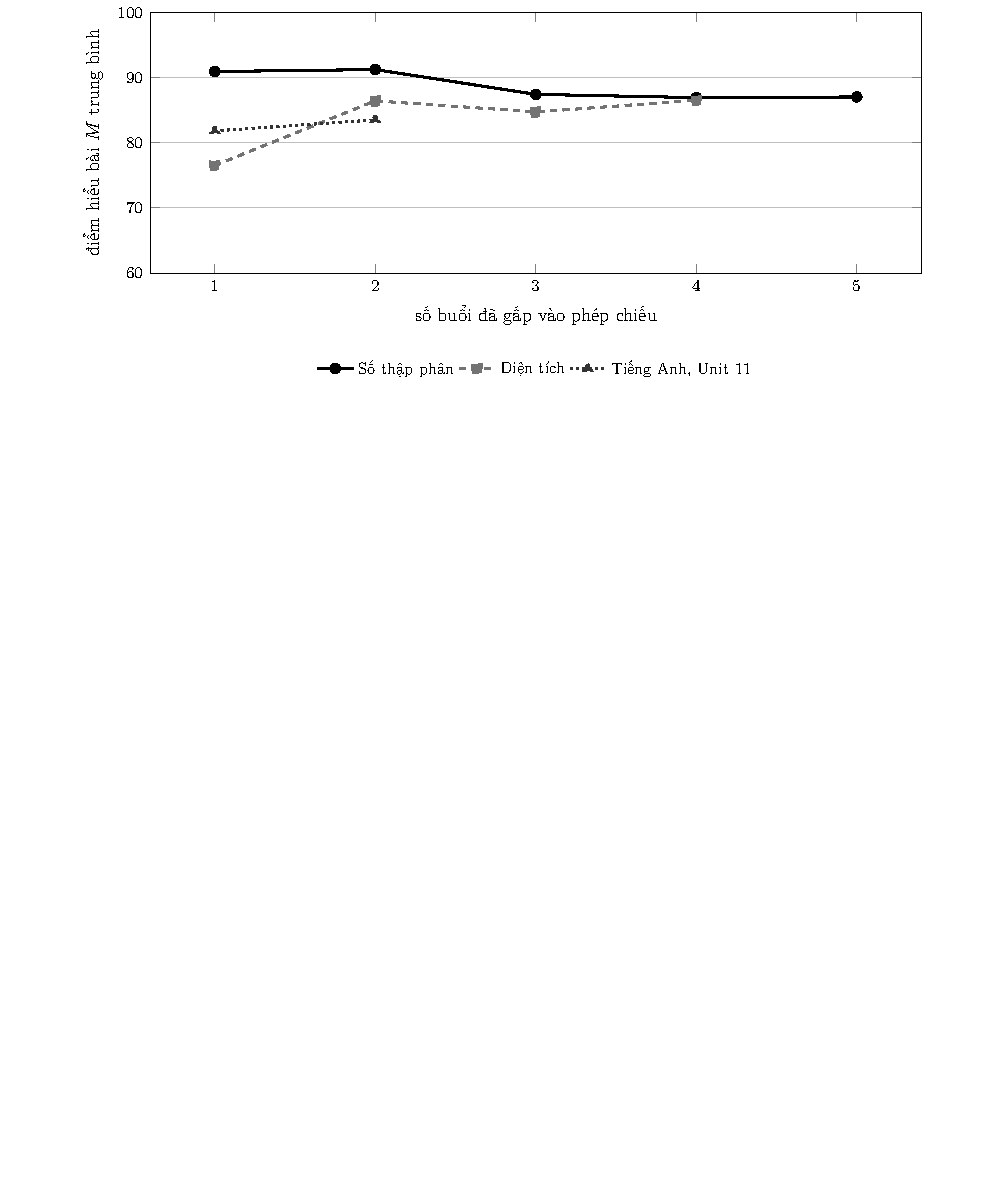
\includegraphics{figures/pdf/fig-db-mastery.pdf}
\caption{Điểm hiểu bài $M$ trung bình sau mỗi buổi được tính vào, tài khoản Vuong, mỗi chương một đường.}
\label{fig:db-mastery}
\end{figure}

\subsection{Kiểm tra công thức và thử với các kiểu học sinh biết trước}
Một công thức có thể đúng về ý nghĩa mà sai khi tính, nên đồ án viết một chương trình đối chứng độc lập tính cùng các đại lượng bằng công thức viết thẳng (cộng trọng số rồi lấy tỉ lệ) thay cho cách cập nhật từng câu. Hệ thống và chương trình đối chứng chạy trên $1\,000$ chuỗi ngẫu nhiên: một nửa là học sinh bất kỳ và một nửa là học sinh khá, học hai buổi cách nhau sáu ngày. Bảng~\ref{tab:learner-conformance} cho kết quả: sai lệch lớn nhất của điểm là $0{,}05$ điểm trên một trăm, nhỏ hơn mức làm tròn hiển thị, không chuỗi nào lệch mức hiểu hay vi phạm thứ tự, giới hạn hoặc điều kiện qua bài, và tính lại cùng chuỗi luôn cho cùng kết quả. Hai dòng cuối của bảng là chỗ điểm đi ngược chiều mong đợi: thêm một bậc gợi ý vào một câu đúng làm điểm tăng ở $6$ trong $500$ chuỗi của học sinh khá (tối đa $6{,}5$ điểm) và thay một câu sai bằng câu đúng làm điểm giảm ở $2$ trong $843$ phép thay (tối đa $2{,}9$ điểm). Đó là hệ quả của quy tắc tự đặt rằng một khía cạnh chỉ được tính khi bằng chứng đạt một lượng tối thiểu, chứ không phải lỗi tính.

% Sinh bởi tools/db_tex.py từ bản sao lưu database; không sửa tay.
\begin{table}[H]
\centering
\caption{Kiểm tương đương giữa phép chiếu mức hiểu và công thức đóng viết độc lập, trên các chuỗi sự kiện ngẫu nhiên}\label{tab:learner-conformance}
\small
\begin{tabular}{p{7.4cm}rr}
\toprule
Chỉ số & Học sinh bất kỳ & Học sinh khá \\
\midrule
Số chuỗi sự kiện & $500$ & $500$ \\
Số sự kiện & $11\,062$ & $13\,116$ \\
Sai lệch lớn nhất của $M$ so với công thức đóng (điểm trên $100$) & $0{,}0499$ & $0{,}0498$ \\
Sai lệch trung bình của $M$ & $0{,}0245$ & $0{,}0249$ \\
Sai lệch lớn nhất của độ tin cậy & $0{,}0500$ & $0{,}0500$ \\
Lệch mức hiểu & $0$ & $0$ \\
Vi phạm thứ tự, phát lại, giới hạn hoặc cổng & $0$ & $0$ \\
Thêm gợi ý mà $M$ tăng & 0/500 & 6/500 \\
Thay câu sai bằng câu đúng độc lập mà $M$ giảm & 1/492 & 1/351 \\
\bottomrule
\end{tabular}
\end{table}


Năm kiểu học sinh do chương trình đóng vai học trọn hai chương Toán, và điểm được kỳ vọng xếp họ theo đúng điều họ được dựng để biết (Bảng~\ref{tab:learner-groups}). Bốn kiểu giỏi, hay sai dạng, hay xin gợi ý và hay sai đều qua mọi bài với điểm từ $91{,}8$ đến $97{,}4$, kiểu hay sai thấp hơn ba kiểu kia khoảng ba điểm. Kiểu phụ thuộc gợi ý, luôn cần gợi ý để làm đúng, không qua bài nào ở cả hai chương với điểm $68{,}7$ và $70{,}7$ và mức hiểu trung bình chỉ $0{,}27$ và $0{,}38$. Hệ thống vì vậy tách được học sinh làm đúng nhờ gợi ý khỏi học sinh làm đúng độc lập nhưng chưa tách được các kiểu còn lại ở mức chi tiết hơn; kiểu hay xin gợi ý trùng điểm với kiểu giỏi vì kịch bản của nó không ghi nhận gợi ý nào trước đáp án đúng.

% Sinh bởi tools/db_tex.py từ bản sao lưu database; không sửa tay.
\begin{table}[H]
\centering
\caption{Điểm hiểu bài mà phép chiếu gán cho năm kiểu học sinh kịch bản đã biết trước}\label{tab:learner-groups}
\small
\begin{tabular}{lrrrrrr}
\toprule
& \multicolumn{3}{c}{Số thập phân} & \multicolumn{3}{c}{Diện tích}\\
\cmidrule(lr){2-4}\cmidrule(lr){5-7}
Kiểu học sinh & Qua bài & $M$ TB & Mức TB & Qua bài & $M$ TB & Mức TB \\
\midrule
Giỏi & 11/11 & $97{,}3$ & $3{,}36$ & 8/8 & $94{,}8$ & $3{,}50$ \\
Hay sai dạng & 11/11 & $97{,}4$ & $3{,}36$ & 8/8 & $94{,}8$ & $3{,}50$ \\
Hay xin gợi ý & 11/11 & $97{,}3$ & $3{,}36$ & 8/8 & $94{,}8$ & $3{,}50$ \\
Hay sai & 11/11 & $94{,}1$ & $3{,}36$ & 8/8 & $91{,}8$ & $3{,}50$ \\
Phụ thuộc gợi ý & 0/11 & $68{,}7$ & $0{,}27$ & 0/8 & $70{,}7$ & $0{,}38$ \\
\bottomrule
\end{tabular}
\end{table}


Các ngưỡng và trọng số không có trong khung gốc được đánh dấu là diễn giải khai báo (DI). Điểm của học sinh do chương trình đóng vai được tính lại hai mươi lần, mỗi lần đổi một diễn giải sang giá trị lân cận. Thay đổi lớn nhất ở chương Số thập phân làm điểm một bài lệch $3{,}2$ điểm, nhiều nhất ba bài đổi mức hiểu trong một lần thay, và $6$ trong $220$ cặp thay đổi đổi kết luận qua bài; ở chương Diện tích là $4{,}5$ điểm, hai bài và $3$ trong $160$ cặp. Kết luận về một học sinh vì vậy khá bền, và chỉ một số ít bài sát ngưỡng đổi trạng thái khi diễn giải đổi.

\subsection{Giới hạn}
Phần tính lại cho biết hệ thống cư xử ra sao trên nhật ký thật của tài khoản thử nghiệm, nhưng chưa cho biết điểm có khớp mức hiểu thật của một đứa trẻ hay không và chưa kiểm khả năng dự báo của mô hình bảy chiều, vì chưa có trẻ em tham gia và chưa có bài kiểm tra độc lập để đối chiếu. Thí nghiệm công thức và kiểu học sinh đóng vai chỉ chứng minh hệ thống tính đúng theo quy tắc đã đặt, không chứng minh quy tắc đúng với việc học. Khía cạnh trí nhớ chưa được đo nên chưa có mức $5$, và các ngưỡng tự đặt chưa được hiệu chỉnh trên dữ liệu của trẻ.
